\section{Wireless Basics}

\begin{figure}[h]
	\centering
	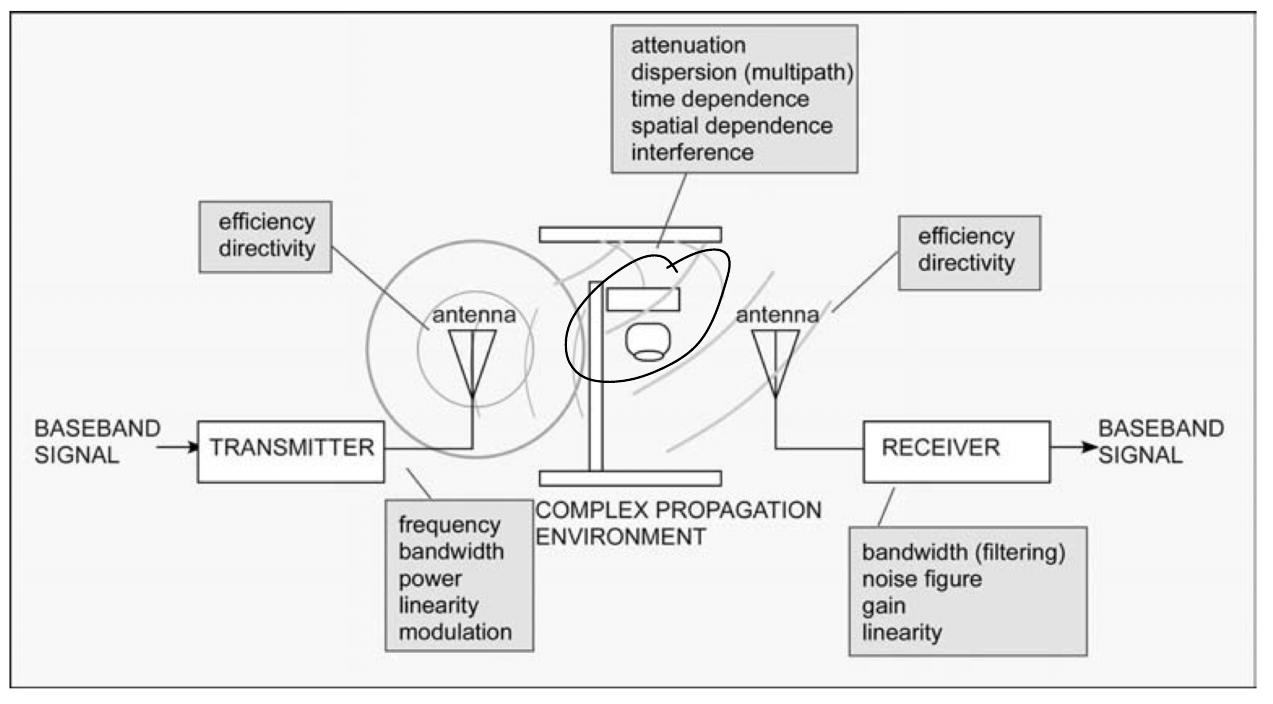
\includegraphics[scale=0.4]{images/1-wireless-system.png}
	\caption{A wireless system, its basic components and characteristic measures}%
	\label{fig:wireless-system}
\end{figure}

\paragraph{Radio Frequency Signal}
Electromagnetic radiation, with waves being created in the antenna by an
alternating current at the desired frequency. Mathematically described as a
function of the time $t$:
\[ v(t) = A \sin (2 \pi f t + \phi) \]
with amplitude $A$, frequency $f$ and phase $\phi$. Also recall that the period
is $T = \frac{1}{f}$ and the wavelength (distance traveled during one period)
is $\lambda = \frac{v}{f}$ (usually $v=c$ speed of light).
The analytic signal is a convenient representation of generic signals in terms of amplitude and phase in the complex domain.
More intuitively, the signal is seen as a vector in the complex plane, the norm of the vector is the amplitude, the angle is the phase, and the "speed" of rotation is the frequency.

\paragraph{Bandwidth}
The capacity of a communications link to transmit the maximum amount of data
from one point to another over a connection in a given amount of time (in bits
per second bps). An analogy: The amount of water that can flow through a water
pipe.

In other words, the measure of frequency content of the signal. E.g.\ the human
voice contains frequencies in the range from 30 Hz to 10 kHz, and the bandwidth
of a single 802.11 channel is 22 MHz.

Often the \hl{bandwidth of the base-band and that of the carrier} (and
thus that of the modulated signal) \hl{differ}. For example, see spread spectrum techniques
(\autoref{sec:jamming-resistant-comm}). Low variability of the signal in time
corresponds to a small bandwidth, whereas a high variability corresponds to a
large bandwidth

\begin{figure}[h]
	\centering
	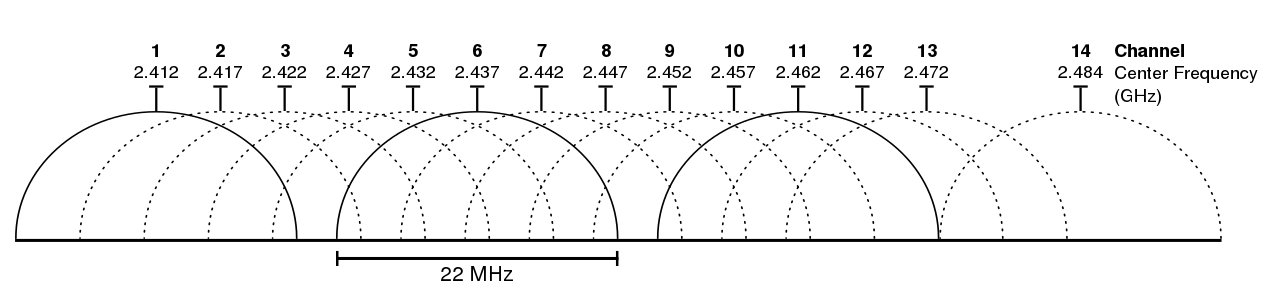
\includegraphics[scale=0.35]{images/1-wifi-channels.png}
	\caption{2.4 GHz WiFi Channels \href{https://en.wikipedia.org/wiki/List\_of\_WLAN\_channels\#/media/File:2.4\_GHz\_Wi-Fi\_channels\_(802.11b,g_WLAN).svg}{[Source]}}%
	\label{fig:wifi-channels}
\end{figure}

\paragraph{Baseband}
A \hl{signal that has not been modulated} or has been
demodulated to its original frequency content, the actual \textbf{information
	signal}. \hl{Telecommunication protocols require base-band signals to be
	up-converted}, or modulated, to a higher frequency in order to be transmitted over
long distances.

\paragraph{Carrier}
A transmitted electromagnetic pulse or wave at a steady base frequency of
alternation on which information can be imposed. Typically \textbf{a pure
	sinusoid of a particular frequency and phase} that will carry the information.
Usually the frequency of the carrier is much higher than that of the baseband.
To go from baseband to passband, we need to multiply the analytic signal with a
carrier, where $f_c$ is the carrier frequency and $a(t)$ is the amplitude.
\[ x_{RF} (t) = \Re \{a(t)e^{i\theta (t)}\} = a(t) \cos (2 \pi f_c t + \theta(t))\]

\subparagraph{Upconversion}
This process is called \textbf{up-conversion}, and it's \hl{necessary mainly for}
two reasons: to \hl{enable simultaneous transmission} of different signals by using
a different carrier frequency (for each transmission) \hl{and to transform a
	complex signal into a real one}, since only real signals can actually be
transmitted. At the receiver, it's then down-converted such that the subsequent
processing can be done in the complex-valued baseband domain.

In order to actually perform the up-conversion, we need an oscillator to
produce the cosine wave at the chosen (carrier) frequency and a mixer to
multiply it with the baseband signal, producing the frequency shift.

\paragraph{Modulated Signal}
A carrier that has been loaded, or modulated, with the information signal.

\paragraph{Modulation}
Process of imposing the baseband onto the carrier. The baseband is used to
alter one or more aspects of the carrier, such as: \hl{signal strength} (\textit{amplitude
	modulation AM}), \hl{frequency} (\textit{frequency modulation FM}), \hl{phase}
(\textit{phase modulation PM}). In other words, one or more of the values $A, f, \phi$
in the above equation of the signal are manipulated.

\paragraph{Amplitude-shift keying ASK}
Modulation technique \hl{varying the amplitude of the signal}.

\paragraph{Frequency-shift keying FSK}
Modulation technique \hl{varying the frequency of the carrier}.

\paragraph{Phase-shift keying PSK}
Modulation technique \hl{varying the phase of the carrier}. It's used, for example,
in WiFi, RFID, Bluetooth. Specific versions include Binary PSK, Quadrature PSK
and Differential PSK.\@ Example: if the baseband bit is 0 do nothing to the
carrier, if it is 1 shift the carrier phase by $\pi$.

\paragraph{On-Off-Keying OOK}
Simple form of amplitude-shift keying ASK.\@ Represents data as the presence
(1) or absence (0) of a signal. E.g.\ Morse code.

\paragraph{I-Q Signal Representation}
A pair of periodic signals are said to be in `quadrature' when they differ in
phase by 90 degrees (e.g.\ the sine and cosine wave). The `in-phase' or
reference signal is referred to as `I' (conventionally cosine), and the signal
that is shifted by 90 degrees (in quadrature) is called `Q' (conventionally
sine). It's used to represent modulations.
\[ I(t) = a(t) \cos (\phi(t)) \leftarrow  \textrm{Analytic signal, } a(t) \textrm{ is the amplitude}\]
\[ Q(t) = a(t) \sin (\phi(t)) \]

\paragraph{Antenna}
Interface between radio waves in the air and electric alternating currents in a
conductor. Types include: omni/dipole, yagi, horn, can-tenna.

The directionality of an antenna described how well it transmits/receives into
a particular direction.
\begin{itemize}
	\item \textbf{isotropic} --- Theoretical, radiates with the same intensity equally in all directions. Often used as a reference antenna when calculating the gain.
	\item \textbf{omnidirectional} --- Radiates equally well in all directions in a flat horizontal plane. Most common types in consumer devices.
	\item \textbf{directional} --- Radiates best in a given direction by focussing its power. Can thus work with weaker signals than an omnidirectional antenna of the same power.
\end{itemize}

\begin{figure}[h]
	\centering
	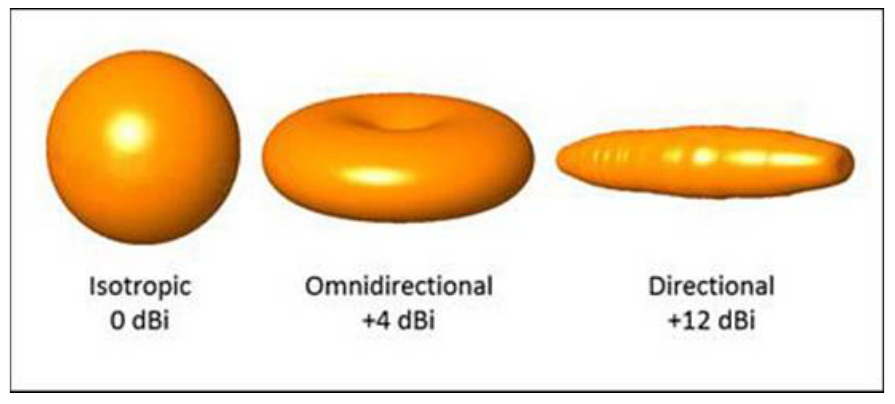
\includegraphics[scale=0.4]{images/1-directionality.png}
	\caption{Antenna directionality}%
	\label{fig:directionality}
\end{figure}

\paragraph{Phased Array}
Array of fixed antennas where \hl{the phase of each signal is dynamically adjusted}
so that the signal will be in phase when viewed from a given direction. \hl{Allows
	\textit{beam steering}} towards a specific direction. Possible applications? Can
it be used to achieve security (e.g.\ confidentiality)?

\begin{figure}[h]
	\centering
	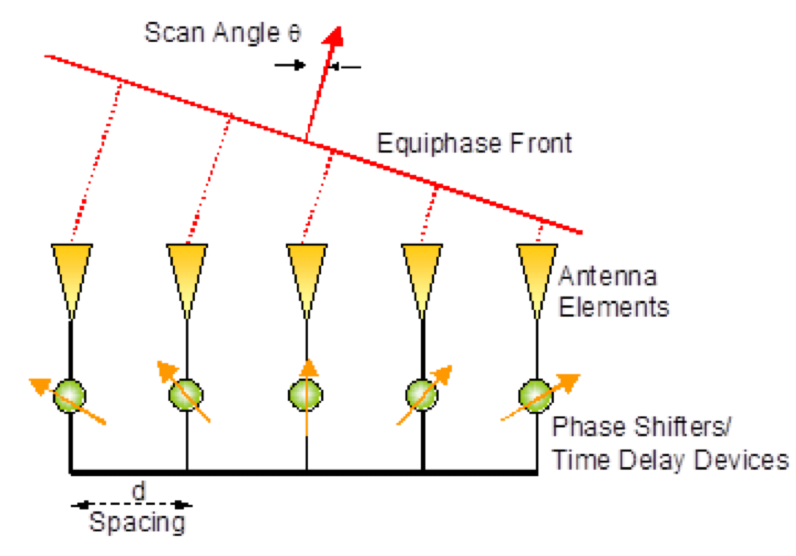
\includegraphics[scale=0.4]{images/1-beam-steering.png}
	\caption{Beam steering}%
	\label{fig:beam-steering}
\end{figure}

\paragraph{Transmitter/Receiver}
They convert the signal from digital to analogue or viceversa, apply de-/modulation and connects to the
antenna. Properties: transmitted power, carrier frequency,
information bandwidth, modulation type, receiver sensitivity.

\paragraph{Software Defined Radio SDR}
Flexible, low-cost transmitter/receiver. Implements components (mixer,
amplifier, de-/modulator) in software rather than processing the signal in
hardware.

\paragraph{Channel equation}

signal strength at the receiver $=$ transm.\ power $+$ transm.\ antenna gain
$-$ link loss $+$ receiv.\ antenna gain

See \autoref{fig:signal-strength}.
Note that, in free space, the power density of an EM wave obeys the
inverse-square law:
\[p \propto \frac{1}{d^2} \]

\begin{figure}[h]
	\centering
	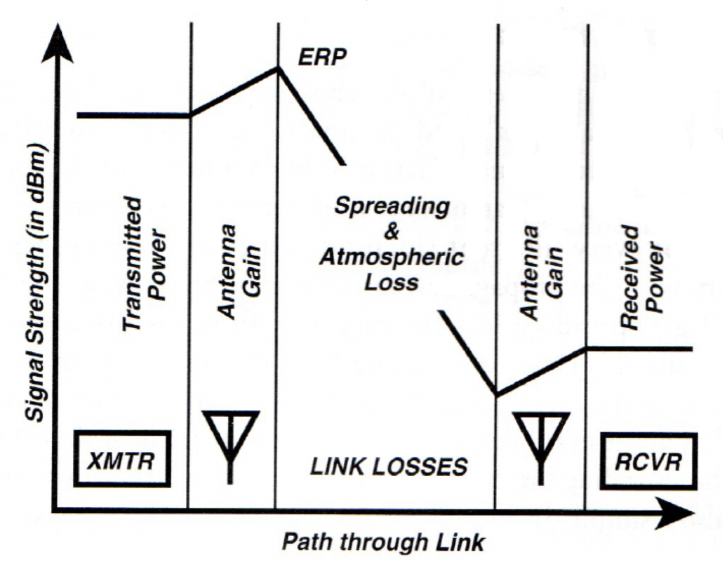
\includegraphics[scale=0.4]{images/1-signal-strength.png}
	\caption{Signal strength across the channel (ERP = Effective Radiated Power)}%
	\label{fig:signal-strength}
\end{figure}

\paragraph{Receiver sensitivity}
The \hl{weakest signal from which the receiver can still obtain the desired
	information} signal. Depends not just on the antenna gain, but also on other
factors such as the noise.

\paragraph{Decibel}
\begin{itemize}
	\item dBm --- signal strength in dB / 1 milliwatt mW
	\item dBW --- signal strength in dB / 1 watt W
	\item dBi --- antenna gain in dB / antenna gain of isotopic antenna in dB
\end{itemize}
Calculating a value in dB \[ dB(n) = 10 \log_{10} (n) \quad \text{ and } \quad dBm(n) = 10 \log_{10} (n / 1 mW) \]

\paragraph{Power Spectral Density diagram}
Depicts the power density (in dB) for a range of frequencies. In simple terms,
it \hl{shows how strong the signal is at a given frequency}.

For a signal $x_T(t)$ defined between $(-\frac{T}{2}, \frac{T}{2})$, its power
in the time domain will be \[P = \lim_{T\rightarrow \infty} \frac{1}{T} \int |x_T(t)|^2 dt \] and its power in the frequency domain will be \[PSD(f) = \lim_{T\rightarrow \infty} \frac{1}{T} \int |X_T(f)|^2 df \]

\paragraph{Security Goals}
Reasons: \textit{security} (integrity, confidentiality, authentication),
\textit{regulatory} (personal liability for misuse of one's network access),
\textit{safety} (RF-enabled implants).

Just reducing transmission power, hoping that the attacker will be too far away
to listen on / send / modify messages, is NOT a solution. In fact, WiFi signals
can be received 10 km away, and similarly Bluetooth at 1 km distance (with
good, directed equipment).

Example: \textit{Passive Keyless Entry and Start systems (PKES)}, i.e.\
wireless car keys. Wrongly assume communication implies physical proximity
(relay attack). Needs: Authenticated proximity verification, message
authentication.

\subsection{Questions}
\textbf{Does a wireless channel, in general, affect all frequencies of a signal equally?} It depends on what kind of noise/interference is present on the channel. If it's general thermal noise, then yes, all frequencies will be generally affected in a similar way. However, if there are other communications happening, then the frequencies used by those transmissions will have a greater noise level.
Also, higher frequency signals suffer from greater attenuation due to the distance traveled compared to lower frequency signals.

\textbf{Which two properties of the wireless channel are leveraged by systems that rely on those for physical-layer based key establishment?} Channel impulse response and received signal strength.
